\documentclass{article}
\usepackage[utf8]{inputenc}
\usepackage[english]{babel}
\usepackage{appendix}

\usepackage{authblk}
\usepackage{minted}

\usepackage{graphicx}
\usepackage{caption}
\usepackage{subcaption}

\graphicspath{ {./img/} }

\usepackage[
backend=biber,
style=alphabetic,
sorting=ynt
]{biblatex}

\addbibresource{bibliography.bib}

\title{Turkish Lira Project report}
\author{Federico Cioschi}
\affil{Università degli Studi di Milano}
\date{February 2021}

\begin{document}

\maketitle

\newpage

\section{Introduction}
This report describes the work I did in order to solve the challenge proposed by the Turkish Lira project \cite{assignment}, assigned during the ``Algorithms for Massive Datasets" course, attended at the ``University of Milan".
The task of the project is to implement from scratch an image classifier based on neural networks using Tensorflow.
In particular, the classifier must take into account the images contained in the ``Turkish Lira Banknote" dataset \cite{dataset} published on Kaggle. The trained classifier must take an image as input and provide as output the corresponding predictions w.r.t. the 5, 10, 20, 500, 100, and 200 lira classes.


\section{Dataset description and preprocessing}
The dataset contains 6000 PNG images of Turkish Lira banknotes and occupies 3.5 GB of memory.
Images are equally divided into 6 subfolders, one for each denomination: 5, 10, 20, 50, 100, 200.
They have a 1280x720 resolution with 3 color channels.
Banknotes are depicted from different perspectives, rotated, with different backgrounds, sometimes folded or covered, sometimes partially out of sight (see Figure \ref{fig:bankonote_5}).

\begin{figure}[h]
    \centering
    \begin{subfigure}[b]{0.45\textwidth}
        \centering
        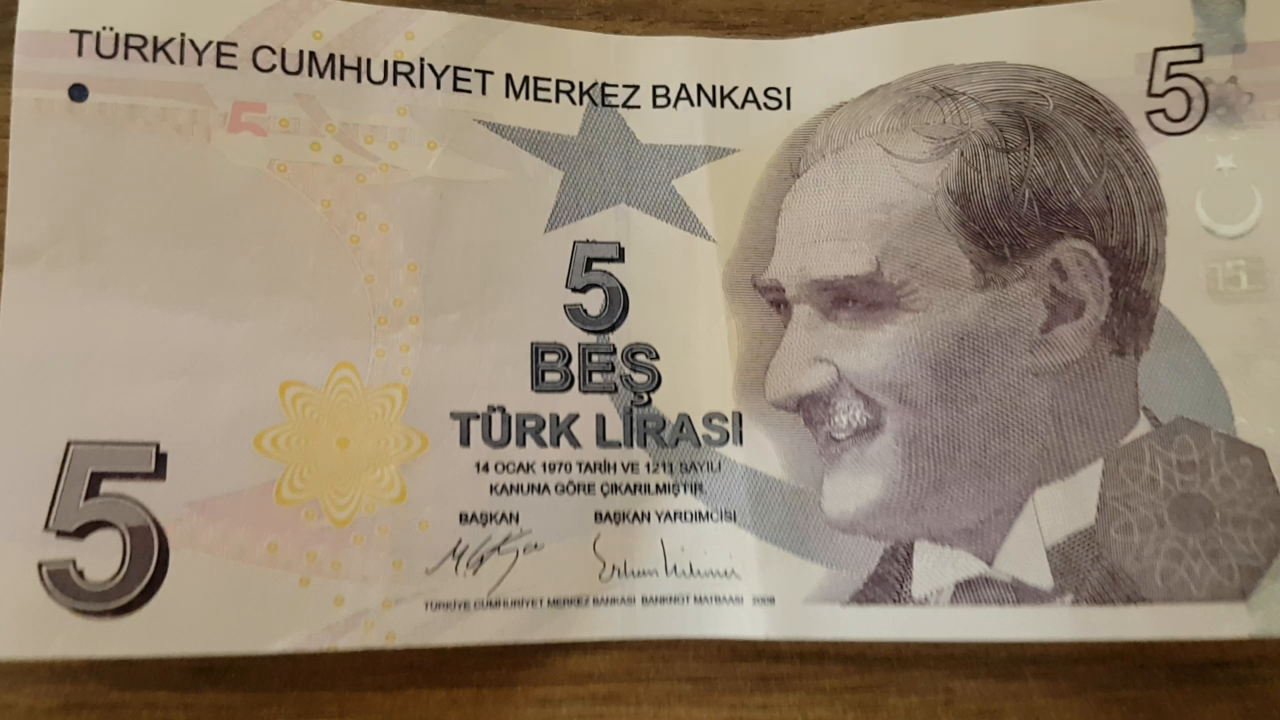
\includegraphics[width=\textwidth]{5_1}
    \end{subfigure}
    \begin{subfigure}[b]{0.45\textwidth}
        \centering
        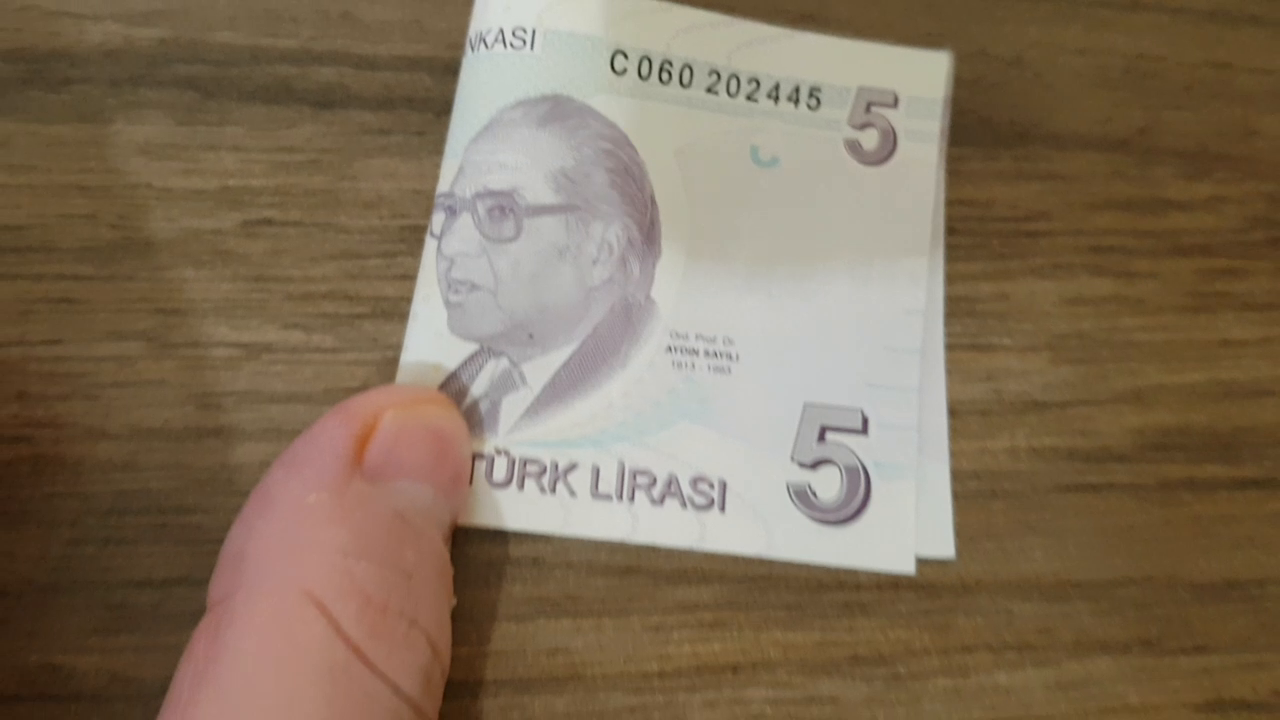
\includegraphics[width=\textwidth]{5_2}
    \end{subfigure}

    \begin{subfigure}[b]{0.45\textwidth}
        \centering
        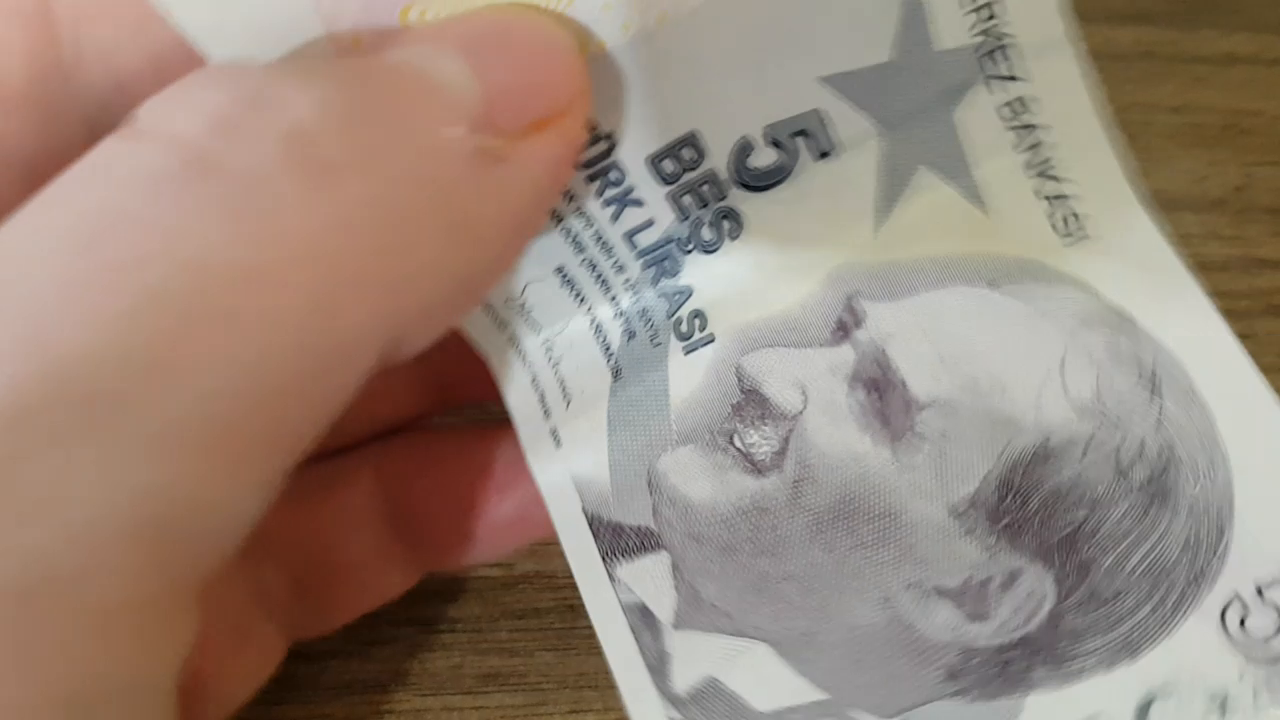
\includegraphics[width=\textwidth]{5_3}
    \end{subfigure}
    \begin{subfigure}[b]{0.45\textwidth}
        \centering
        
\includegraphics[width=\textwidth]{5_4}
    \end{subfigure}
    \caption{Turkish Lira banknotes from different perspectives, rotated, with different backgrounds, sometimes folded or covered, sometimes partially out of sight.}
    \label{fig:bankonote_5}
\end{figure}

\noindent Various data augmentation techniques were already applied by the author to enlarge the dataset \cite{dataset}: brightness increasing and decreasing, image flipping, salt-and-pepper noise addition (see Figure \ref{fig:bankonote_10}).
\begin{figure}[h]
    \centering
    \begin{subfigure}[b]{0.3\textwidth}
        \centering
        
\includegraphics[width=\textwidth]{10}
    \end{subfigure}
    \begin{subfigure}[b]{0.3\textwidth}
        \centering
        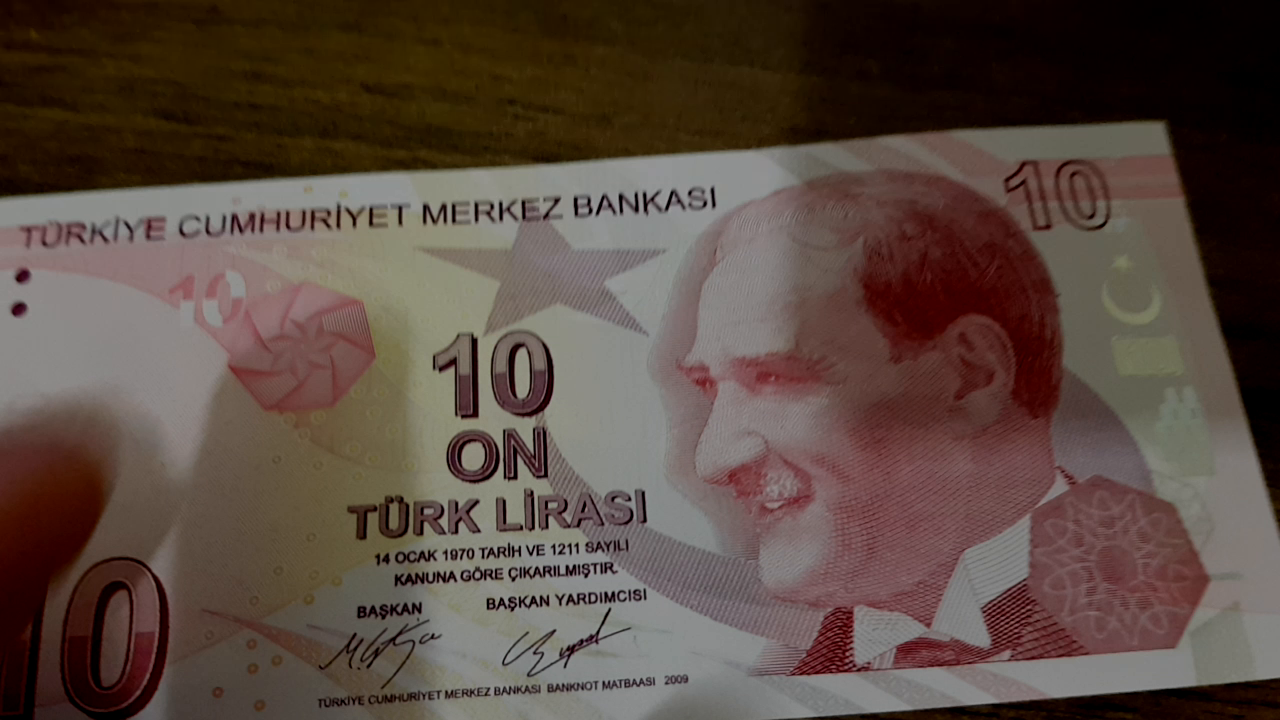
\includegraphics[width=\textwidth]{10_eminus}
    \end{subfigure}
    \begin{subfigure}[b]{0.3\textwidth}
        \centering
        
\includegraphics[width=\textwidth]{10_eplus}
    \end{subfigure}
    
    \begin{subfigure}[b]{0.45\textwidth}
        \centering
        
\includegraphics[width=\textwidth]{10_flipped}
    \end{subfigure}
    \begin{subfigure}[b]{0.45\textwidth}
        \centering
        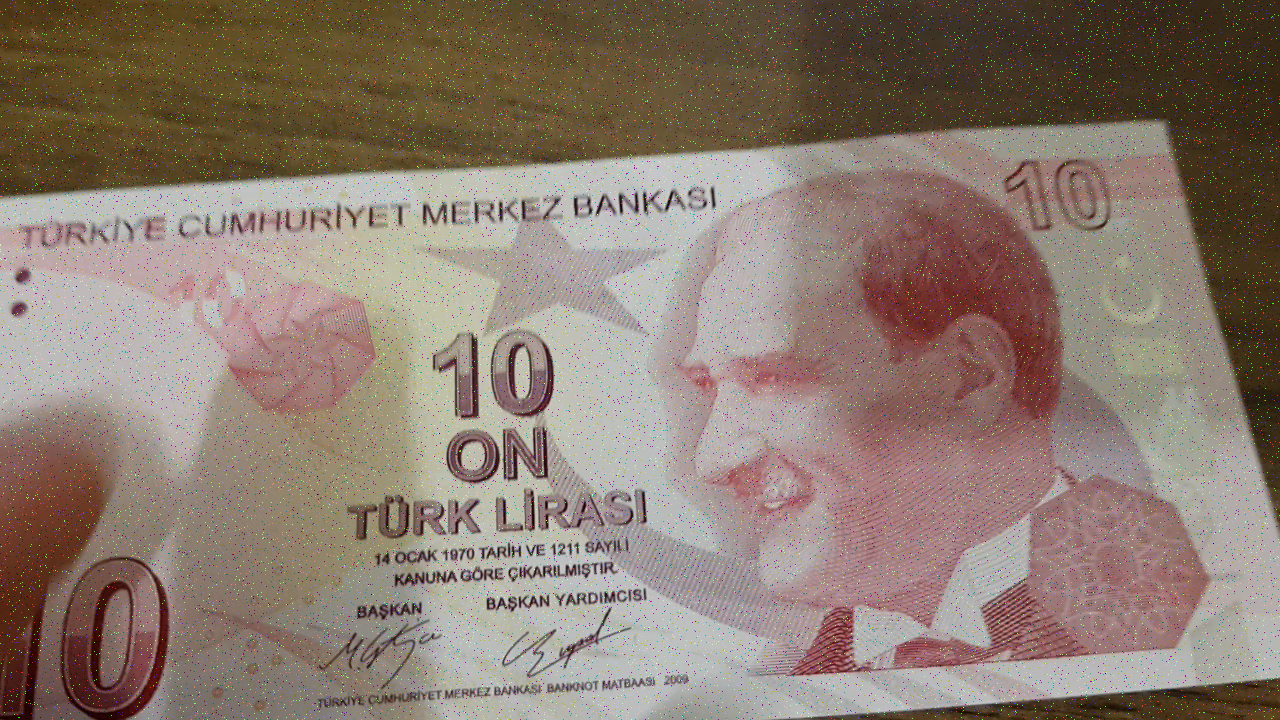
\includegraphics[width=\textwidth]{10_saltAndPeppered}
    \end{subfigure}
    \caption{Turkish Lira banknotes with brightness decreased or increased, flipped, salt-and-peppered.}
    \label{fig:bankonote_10}
\end{figure}

I used the \texttt{tf\-.keras\-.pre\-pro\-ces\-sing\-.image\_\-dataset\_\-from\_\-directory} function to create a \texttt{tf\-.data\-.Dataset} object for both the training dataset and the validation dataset.
Moreover, this function preprocessed the images resizing them to the resolution of 64x64 and then converting them into \texttt{(64,64,3)} tensors.
Training dataset was composed by the 80\% of the images in the original dataset, while the remaining 20\% constituted the validation dataset.
During training, images from the training dataset were provided to the model in batch of 100 items at a time.
Finally, the first layer of each model which I defined in this project re-scales the RGB values from the $[0,255]$ range to the range $[0,1]$, which is better for neural networks processing.

\section{Network Architecture and Implementation}
\label{architecture}

I addressed the project task using Convolutional Neural Networks (CNN).
CNNs are feed-forward deep neural networks which have revealed to be very good and efficient for image classification.
In order to implement CNNs, I employed the open source library TensorFlow, as requested by the project task.

As stated in \cite{cnnStanford}, the most common architectures for CNNs follows this pattern:
\begin{verbatim}
INPUT -> [[CONV -> RELU]*N -> POOL?]*M -> [FC -> RELU]*K -> FC
\end{verbatim}
CONV, followed by RELU, represents a convolutional layer which neurons use the ReLU activation function.
POOL instead, represents a pooling layer.
Finally FC, followed by RELU, represents a fully connected layer which neurons use the ReLU activation function.

The main idea of this architecture is to alternate convolutional layers with pooling layers:
the former are responsible for collecting and filtering information from the input, while the latter are responsible for aggregating this information and therefore reducing the spatial dimension of the input.
Finally, everything is flattened and processed by one or more fully connected layers, which leads the network to calculate the final classification.

\subsection{Input size}
Typically in CNNs the width and the height of the input are equal and corresponds to an integer divisible by 2 several times.
Indeed pooling layers usually halves the width and the height of the input, de facto reducing by a factor 4 its the spatial dimension.
As suggested in \cite{cnnStanford}, CNNs should repeatedly reduce the spatial dimension through pooling layers until the image has been merged spatially to a small size.

After a bit of tweaking, I found that the best trade-off, in order to have powerful CNNs on one side and to limit their complexity on the other side, was to set the initial input size to 64x64: in this way the input size, after \texttt{M=3} pooling operations, is shrinked to a size of 8x8.
This is the reason why, during preprocessing, images are resized to the 64x64 resolution.

\subsection{Layers Depth}
Layers in CNNs do not expand only in height and width, but also in depth.
Obviously the depth of the first layer is only 3, because it reflects the size of the images given as input to the network; indeed images are encoded as \texttt{(64, 64, 3)} tensors, because each pixel is described by three RGB values.
However, in the following layers, the depth corresponds to the number of neurons which act as filters on the same receptive field.
A typical pattern is to double the number of filters after each pooling layer.
The increasing number of filters in deeper layers of the network is justified by the fact that neurons in these layers are responsible for bigger regions of the original input image: so they have to activate themselves in presence of a larger number of shapes that could appear in that region.
In this project, I set to 32 the depth of the layers in the first ``\texttt{[CONV -> RELU]*N -> POOL]}" block.
Since \texttt{M=3}, then I doubled the depth two times: thus, the second block has layers with 64 filters and the third one has layers with 128 filters.

\subsection{Convolutional Layers}
Commonly, before a pooling layer, more convolutional layers may be stacked together.
As explained in \cite{cnnStanford}, it is better to stack together some convolutional layers with a small filter size, than having a singular convolutional layer with a big filter size.
This allows to the network to capture more powerful features of the input with fewer parameters.

For these reasons, I set the filter size (\texttt{kernel\_size} in TensorFlow) of the convolutional layers to 3x3.
Moreover, since convolutional layers are not meant to reduce the spatial dimension of the input, I set stride to 1 and I enabled padding.

I have not fixed the number \texttt{N} of convolutional layers to be stacked together.
Indeed, I evaluated the performance of the network for different values of \texttt{N}, see Section \ref{experiments}.


\subsection{Pooling Layers}
I used TensorFlow \texttt{MaxPooling} to implement pooling layers.
Since pooling layers have the purpose to reduce the spatial dimension of the input, I set their filter size (\texttt{pool\_size} in TensorFlow) to 2x2; moreover I set their stride to 2 and I disabled padding.
This setting, suggested in \cite{cnnStanford}, allows to the pooling layers to reduce the spatial dimension of the input of 75\%.

\subsection{Final layers, loss function and optimizer}
I set parameter \texttt{K} to \texttt{1}, so CNNs implemented in this project have only one fully connected layer before the output layer.
This layer has 90 neurons with a ReLU activation function.
This setting has revealed to be able to reach optimal results, so I did not take into account other solutions.

The output layer uses the \texttt{softmax} activation function, which is useful to highlight the winning class and also to interpret the network output as a probability distribution.

Moreover, as loss function I used \texttt{cate\-gorical\_cross\-entropy}, which is the most effective for classification problems \cite{cross_entropy}.

Finally, I used \texttt{Adam} as optimizer, which is an extension of the classical Stochastic Gradient Descent method that uses moments to avoid to get stuck in saddle points during training.
As \texttt{learning\_rate} parameter in \texttt{Adam}, I used \texttt{0.01}.

\section{Scalability}
The dataset used for this project takes up only 3.5 GB of memory. For this reason I saved it entirely in local storage.
Then, I called the \texttt{tf\-.keras\-.pre\-pro\-ces\-sing\-.image\_\-dataset\_\-from\_\-directory} function to create a \texttt{tf.data.Dataset} object from image files in the dataset directory.
This object was useful to load batches of images from storage to main memory during training and validation.
If the dataset was larger, I could save it on a distributed file system.
At that point, the dataset path in the distributed file system could be past similarly to \texttt{image\_\-dataset\_\-from\_\-directory}, as if it were a local path.
For this reason, the solution I used would have no problem dealing with larger datasets.

In order to efficiently load dataset images from disk to memory, I called two important functions on the \texttt{tf.data.Dataset} object \cite{tfPerformance}:
\begin{itemize}
    \item \texttt{cache}, which keeps images in memory after they have been loaded from disk; if the dataset is too large to fit into memory this method can also create a performant cache-file on disk;
    \item \texttt{prefetch}, which allows to overlap current training step with data loading for the next training step.
\end{itemize}

Finally, I defined all the CNNs in this project under the \texttt{Multi\-Worker\-Mirrored\-Strategy}, which allows to synchronously distribute training across multiple GPUs, hosted on multiple computers  \cite{distr_training_guide}, \cite{distr_training_blog}, \cite{distr_training_tutorial}.
This means that each training batch is potentially divided in slices distributed to the available GPUs, each of which in sync processes the assigned input slice and then aggregate the obtained results with those of the other GPUs.
Implementing this solution in TensorFlow was really simple.
The only things I had to do were to declare the strategy and then to define model under that strategy.
For example:
\begin{minted}{python}
strategy = tf.distribute.MultiWorkerMirroredStrategy()
with strategy.scope():
    model = tf.keras.Sequential()
    model.add( ... )
    ...
\end{minted}
This allowed to TensorFlow to automatically detect all the GPUs available on the local machine.
Moreover, it is possible to inform TensorFlow about the availability of other remote devices configuring the \texttt{TF\_CONFIG} environment variable.
This variable is a JSON string declaring the IP addresses of the other devices and their tasks.
An example of configuration, from \cite{distr_training_guide}, is:
\begin{minted}{python}
os.environ["TF_CONFIG"] = json.dumps({
    "cluster": {
        "worker": ["host1:port", "host2:port", "host3:port"],
        "ps": ["host4:port", "host5:port"]
    },
   "task": {"type": "worker", "index": 1}
})
\end{minted}

\noindent All the experiments done for this project were run using only one GPU, the one offered by the Google Colab environment.
However, the code implementation is completely compatible with distributed training.


\section{Experiments and Results}
\label{experiments}

\subsection{Experiments}
As discussed in Section \ref{architecture}, I took into account the following architecture in order to build the requested CNN:
\begin{verbatim}
INPUT -> [[CONV -> RELU]*N -> POOL]*M -> [FC -> RELU]*K -> FC
\end{verbatim}
As already justified in Section \ref{architecture}, I fixed \texttt{M=3} and \texttt{K=1}.
Contrary, I decided to experiment CNN performances for different values of \texttt{N}, in particular \texttt{1,2,3}.
Moreover, doing preliminary attempts, I found that optimizations like the addition of Batch Normalization layers, or the scheduling of an epoch-dependent upper limit for the Learning Rate Decay, could greatly improve network performances.
For these reasons I decided to execute 9 experiments, summarized here:
\begin{itemize}
    \item testing of a basic architecture for each value of \texttt{N=1,2,3}
    \item testing of an architecture with Batch Normalization, for each value of \texttt{N=1,2,3}
    \item testing of an architecture with Batch Normalization and scheduling of Learning Rate Decay, for each value of \texttt{N=1,2,3}
\end{itemize}

\noindent In particular, in order to reduce the Learning Rate at each epoch, I used the following lambda function (also plotted in Figure \ref{fig:lr_decay}):
\begin{minted}{python}
    lambda epoch: 0.01 * math.pow(0.8, epoch)
\end{minted}
which is applied to the model through the \texttt{tf\-.keras\-.callbacks\-.Learning\-RateScheduler} callback.

\begin{figure}
    \centering
    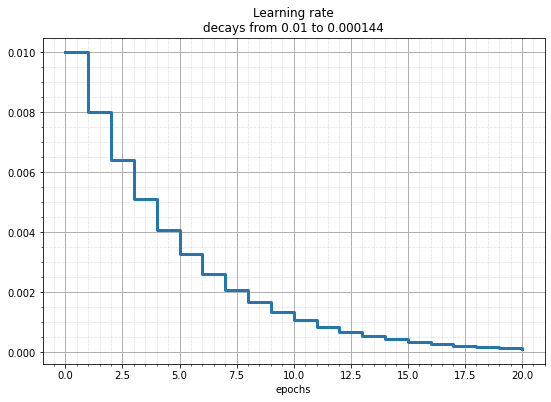
\includegraphics[width=0.5\textwidth]{lr_decay}
    \caption{Learning Rate Decay}
    \label{fig:lr_decay}
\end{figure}

\noindent Basically models are trained for 20 epochs, but I defined two callbacks for early-stopping:
\begin{itemize}
    \item \texttt{no\_learning\-\_early\_stopping\_callback}, which stops training if training accuracy is under $30\%$ for 5 consecutive epochs, as a symptom that model is not learning (continuing training would be pointless);
    \item \texttt{max\_accuracy\-\_early\-\_stopping\-\_callback}, which stops training if both training accuracy and validation accuracy are $100\%$ for 2 consecutive epochs, in order to avoid overfitting once a so good result has been achieved.
\end{itemize}

\noindent A possible optimization which I did not take into account is the addition of a Dropout layer.
However, as shown in Subsection \ref{results}, various models achieved optimal results even without Dropout, so I decided to not take it into account.

The experiments were conducted in the Google Colab environment, which provides:
\begin{itemize}
    \item CPU: Intel(R) Xeon(R) CPU @ 2.20GHz
    \item GPU: Tesla T4
    \item RAM: about 13 GB
\end{itemize}

\subsection{Results}
\label{results}
Appendix \ref{app:accuracy} shows aggregated results for training and validation accuracy, while Appendix \ref{app:loss}, shows aggregated results for training and validation loss.
Notice that graphs in Figures \ref{fig:accuracy_general} and \ref{fig:loss_general} show the same results of graphs in Figures \ref{fig:accuracy_zoomed} and \ref{fig:loss_zoomed}, but they are zoomed when possible.

As shown in Figure \ref{fig:accuracy_general}, among the models which do not use batch Normalization and Learning Rate Decay, only the one with parameter \texttt{N=1} succeeded in learning significantly within the first 5 epochs.
Indeed, the other two models were stopped by the
\texttt{no\_learning\-\_early\_stopping\_callback}.
Despite the model with \texttt{N=1} reached the maximum value of training accuracy, it did not happen the same for validation accuracy, indicating a bit of overfitting.

The introduction of Batch Normalization certainly introduced a big improvement.
All the models which use Batch Normalization succeeded in learning and they also achieved maximum or almost-maximum values for accuracy, both in training and in validation.
Among them, the best is certainly the one with parameter \texttt{N=1}, which indeed was stopped by \texttt{max\_accuracy\-\_early\-\_stopping\-\_callback} at epoch 14, after having maintained the maximum training and validation accuracy for two consecutive epochs.
Also the model with parameter \texttt{N=2} obtained the same result, but only at epoch 20 and after wide fluctuations in both training and validation accuracy.
Probably, those fluctuations were caused by too large \texttt{Adam}'s learning rate parameters which prevented accuracy and loss to converge towards their best values.
Finally, the model with parameter \texttt{N=3} has a very strong gap between training and validation accuracy, signaling overfitting.

The introduction of Learning Rate Decay provided big additional improvements to models performance.
The fluctuations in accuracy and loss are almost absent, except a bit in model with parameter \texttt{N=3}.
Both the models with parameter \texttt{N=1} and \texttt{N=2} were early stopped by \texttt{max\_accuracy\-\_early\-\_stopping\-\_callback}, the second one even at epoch 11.

\begin{figure}[H]
    \centering
    \begin{subfigure}[b]{0.45\textwidth}
        \centering
        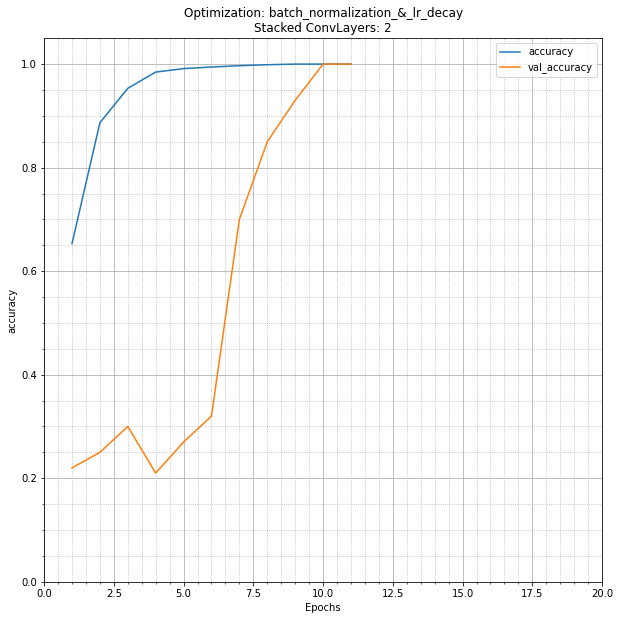
\includegraphics[width=\textwidth]{best_model_accuracy}
    \end{subfigure}
    \begin{subfigure}[b]{0.45\textwidth}
        \centering
        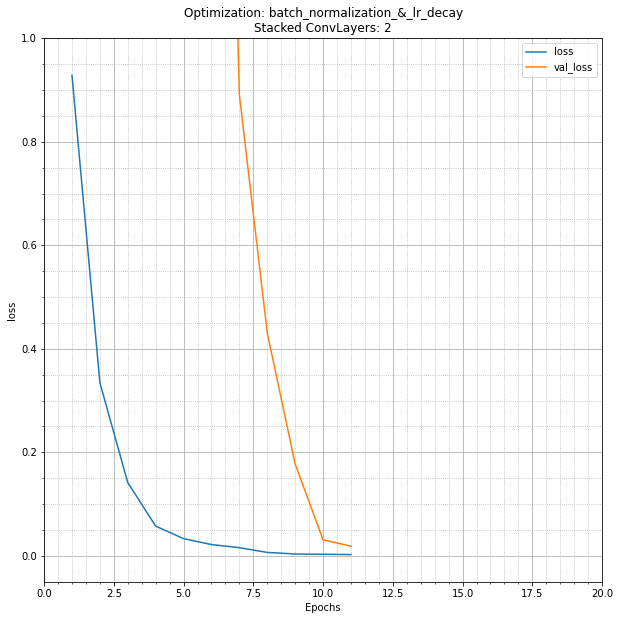
\includegraphics[width=\textwidth]{best_model_loss}
    \end{subfigure}
    \caption{Best model, accuracy and loss graphs.}
    \label{fig:best_model_graphs}
\end{figure}

The model with Batch Normalization, Learning Rate Decay and parameter \texttt{N=2} was the quicker to converge and to be early stopped.
According to its graphs, accuracy and loss converged to their best values very quickly and also without fluctuations; this happened both in training and in validation.
Its training required only 17 minutes and 32.01 seconds.
For these reasons, I think that this model is the best between all.
Its architecture is shown in Figure \ref{fig:best_model_arch}, and its accuracy and loss graphs are singularly shown in Figure \ref{fig:best_model_graphs}.

It should be noted that also two models with parameter \texttt{N=1}, the one with Learning Rate Decay and the one without it, achieved excellent results.

\newpage

\appendix

\section{Accuracy Results}
\label{app:accuracy}

\subsection{Accuracy: General View}
\begin{figure}[h]
    \centering
    \centerline{
        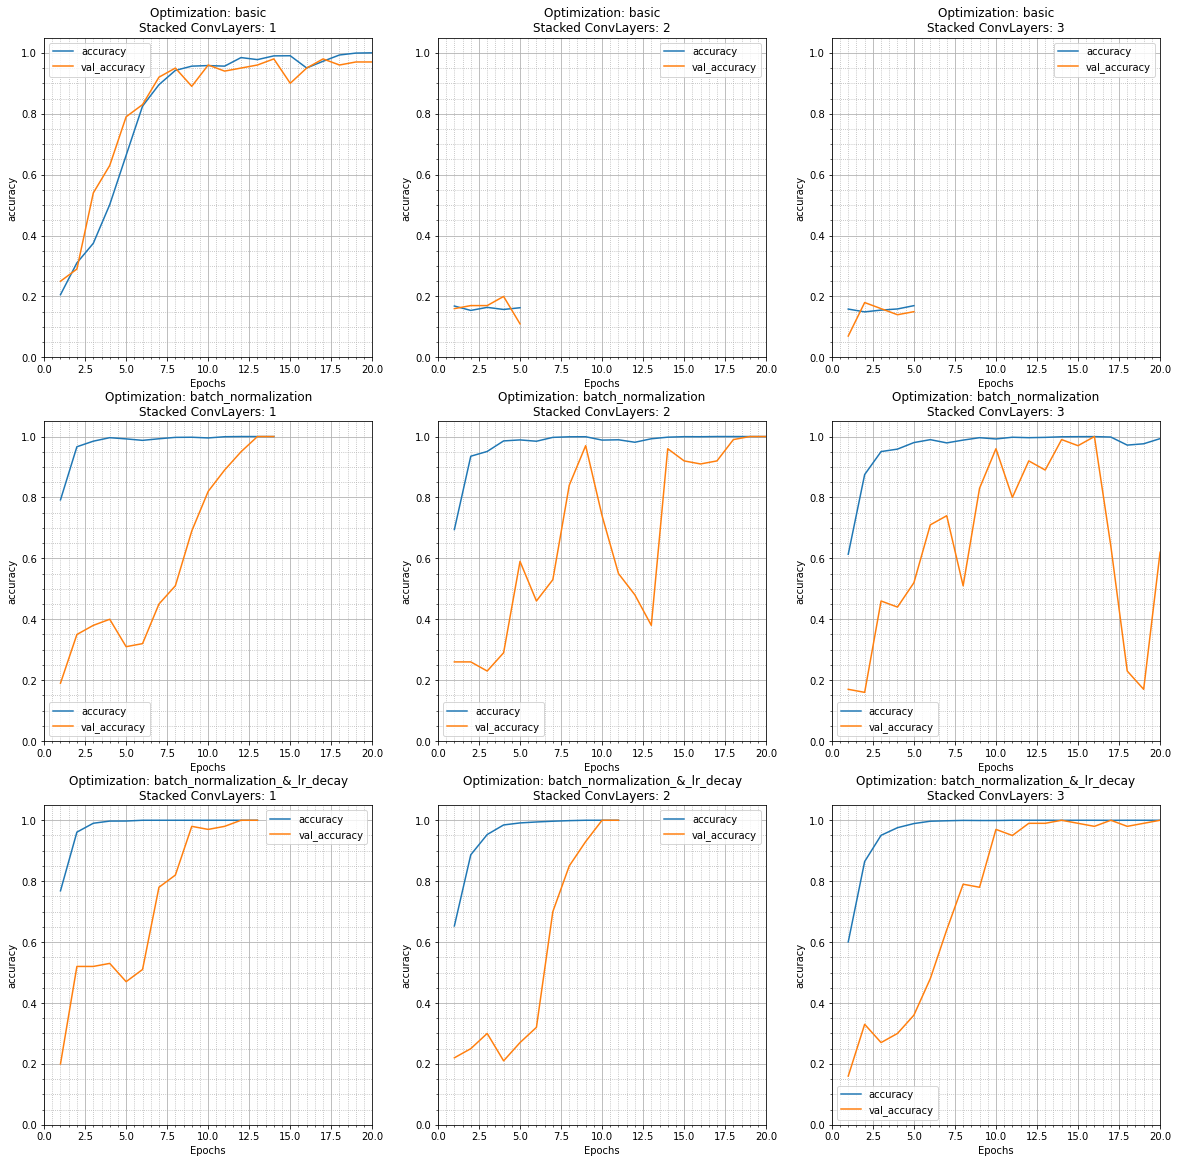
\includegraphics[width=0.65\paperwidth]{accuracy_general}
    }
    \caption{General view of accuracy results; all graphs have the same scale.}
    \label{fig:accuracy_general}
\end{figure}


\newpage

\subsection{Accuracy: Zoomed View}
\begin{figure}[h]
    \centering
    \centerline{
        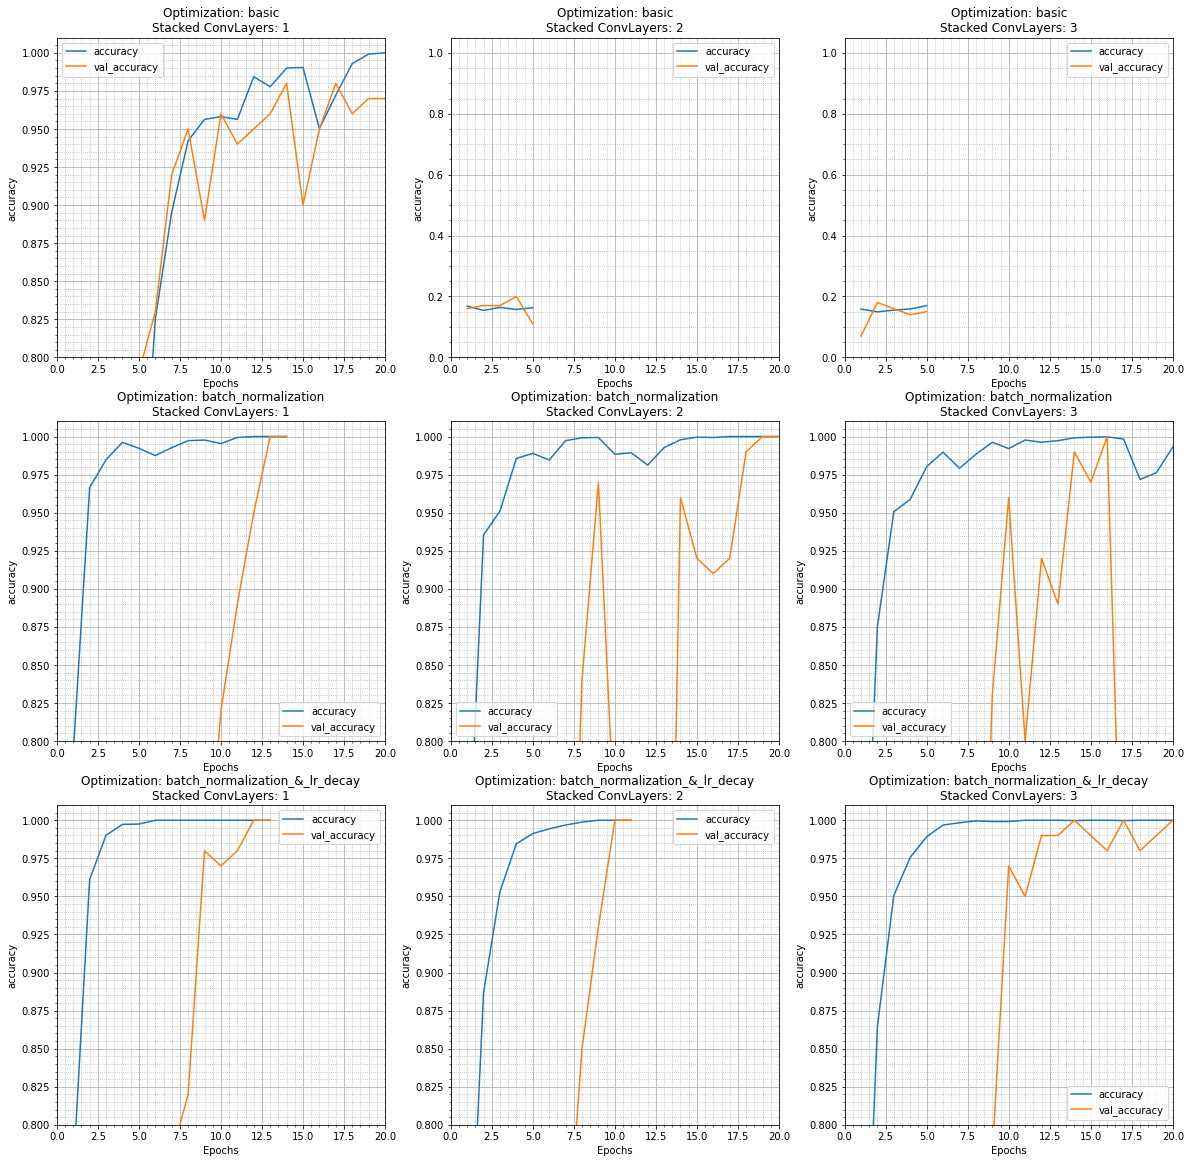
\includegraphics[width=0.65\paperwidth]{accuracy_zoomed}
    }
    \caption{Zoomed view of accuracy results; all, except the two graphs in the upper right corner, are zoomed in by a factor of 5.}
    \label{fig:accuracy_zoomed}
\end{figure}

\newpage

\section{Loss Results}
\label{app:loss}

\subsection{Loss: General View}
\begin{figure}[h]
    \centering
    \centerline{
        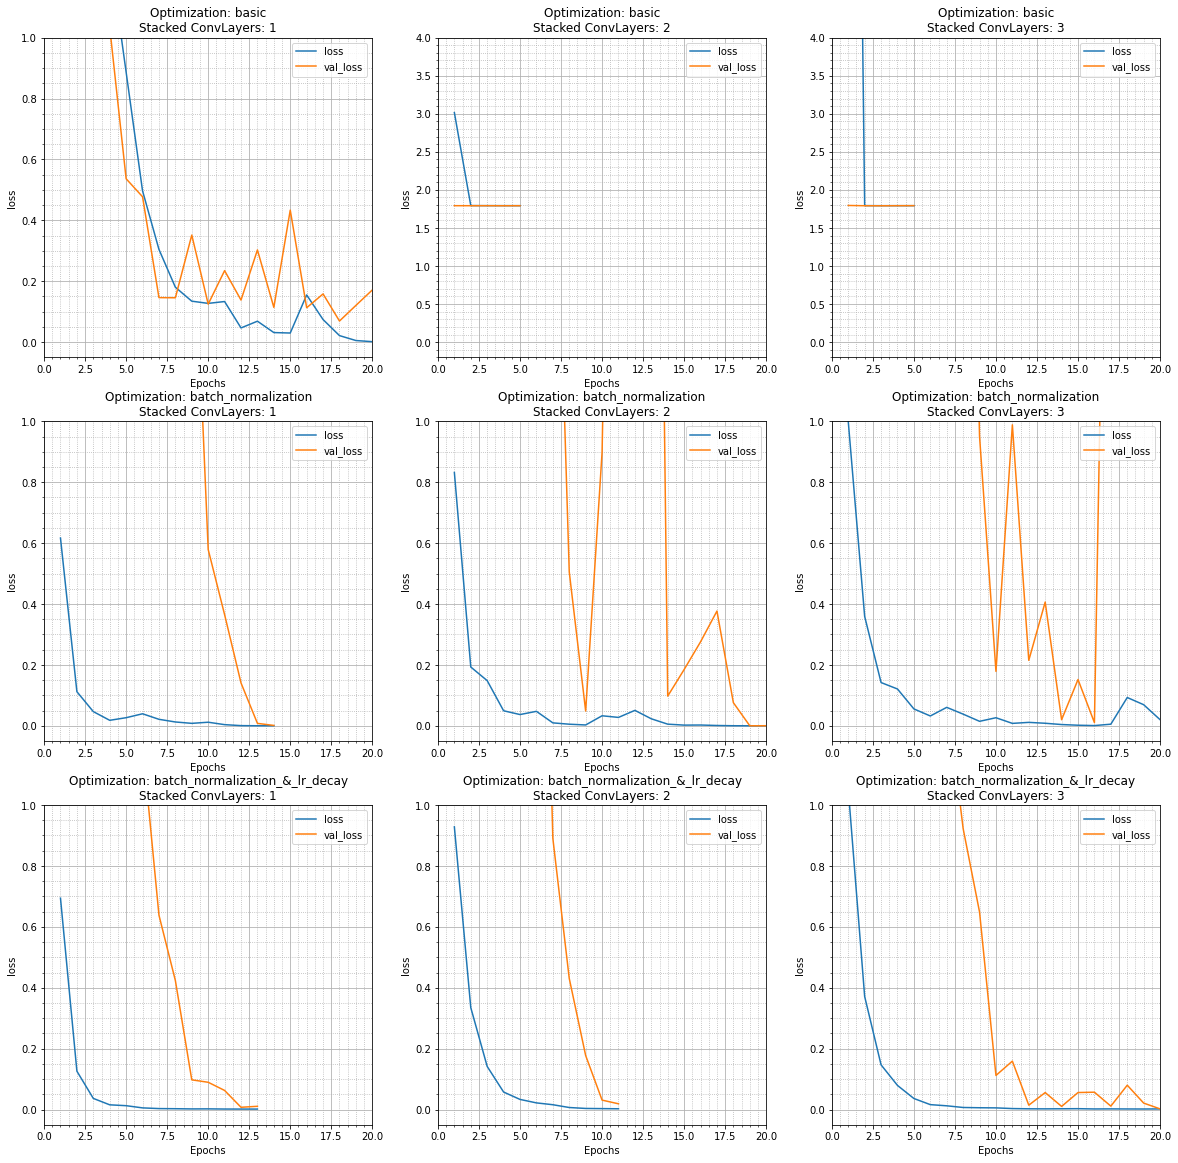
\includegraphics[width=0.63\paperwidth]{loss_general}
    }
    \caption{General view of loss results; all graphs, except the two graphs in the upper right corner, have the same scale.}
    \label{fig:loss_general}
\end{figure}


\newpage

\subsection{Loss: Zoomed View}
\begin{figure}[h]
    \centering
    \centerline{
        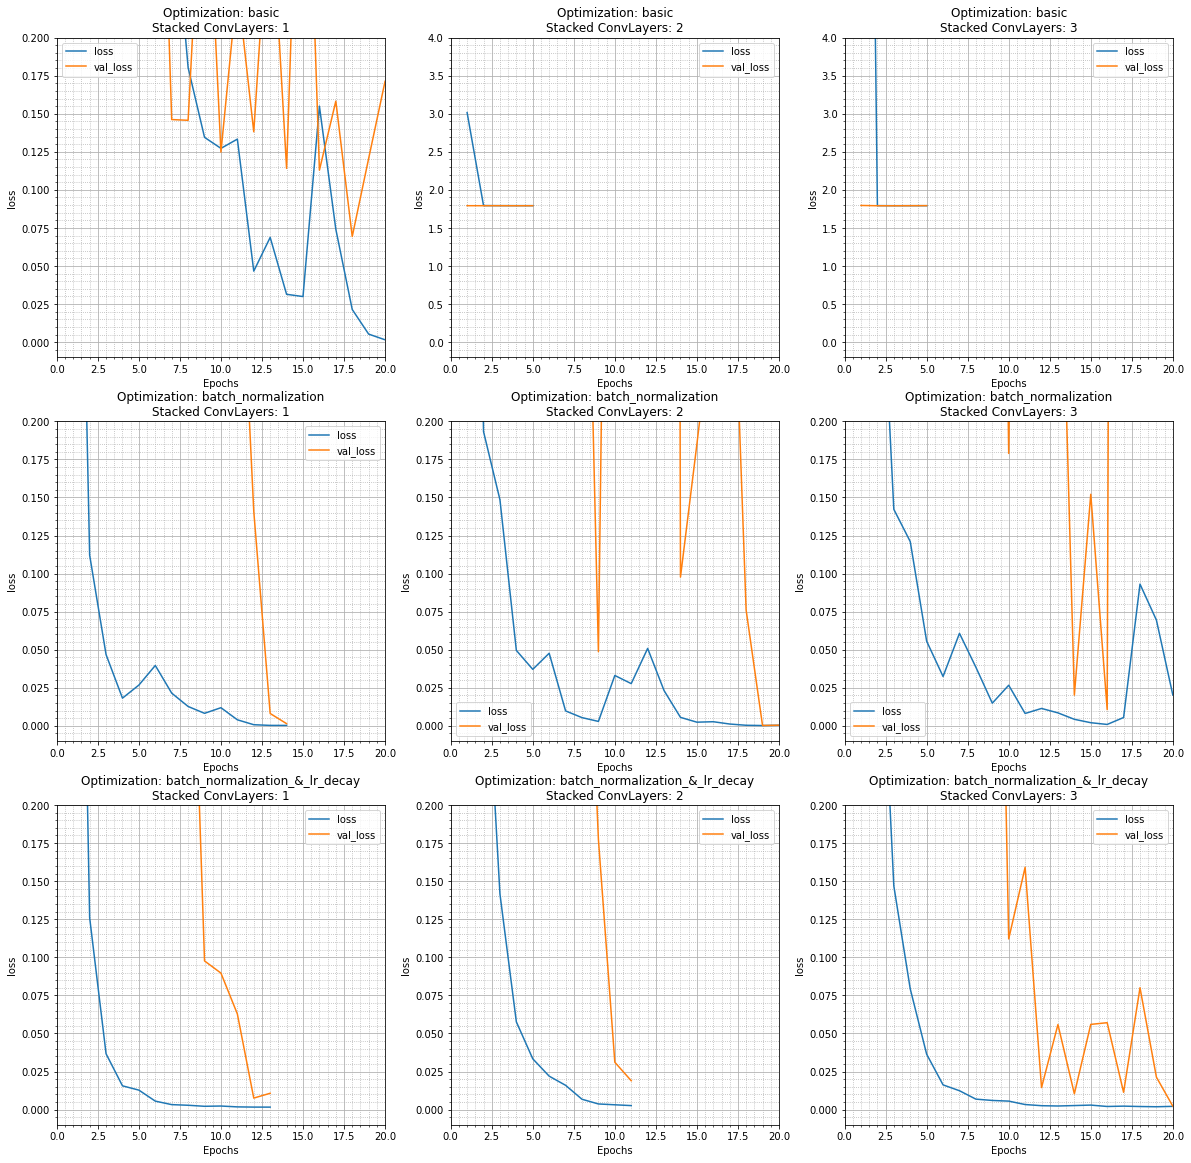
\includegraphics[width=0.65\paperwidth]{loss_zoomed}
    }
    \caption{Zoomed view of loss results; all, except the two graphs in the upper right corner, are zoomed in by a factor of 5.}
    \label{fig:loss_zoomed}
\end{figure}

\newpage

\section{Best Model}
\begin{figure}[h]
    \centering
    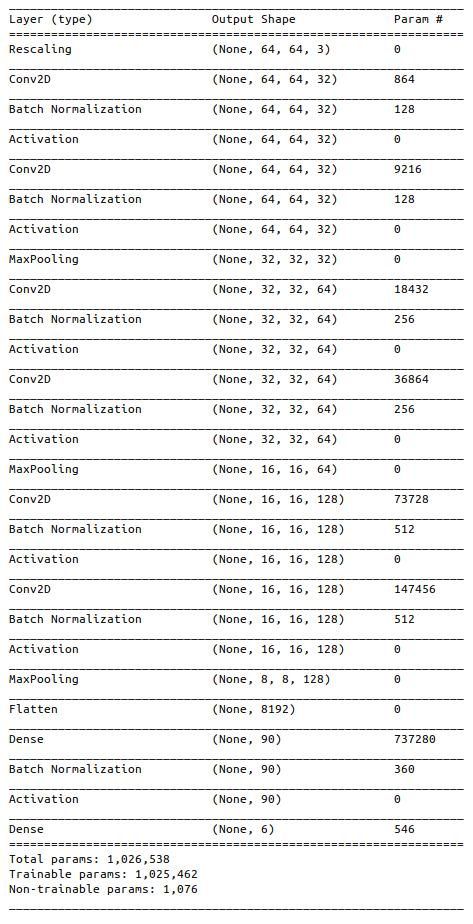
\includegraphics[height=0.7\textheight]{best_model_arch}
    \caption{Best model architecture: \texttt{INPUT -> [[CONV -> RELU]*2 -> POOL]*3 -> FC -> RELU -> FC}}
    \label{fig:best_model_arch}
\end{figure}

\newpage

\printbibliography

\newpage

\noindent \textit{I declare that this material, which I now submit for assessment, is entirely my own work and has not been taken from the work of others, save and to the extent that such work has been cited and acknowledged within the text of my work. I understand that plagiarism, collusion, and copying are grave and serious offences in the university and accept the penalties that would be imposed should I engage in plagiarism, collusion or copying. This assignment, or any part of it, has not been previously submitted by me or any other person for assessment on this or any other course of study.}

\end{document}
